\documentclass[12pt, a4paper]{article}

% --- Packages ---
\usepackage[utf8]{inputenc}    % Language support
\usepackage[margin=1in]{geometry} % Page margins
\usepackage{graphicx}          % To include screenshots of your dashboard
\usepackage{booktabs}          % Professional tables
\usepackage{hyperref}          % For clickable links (GitHub/Streamlit)
\usepackage{xcolor}            % For color coding
\usepackage{listings}
\usepackage{float}
\usepackage{amsmath}
\usepackage[scaled]{helvet}
          

% Define your project color
\definecolor{CoffeeGreen}{HTML}{85BB65}

\hypersetup{
	colorlinks=true,
	linkcolor=black,
	urlcolor=CoffeeGreen,
	pdfborder={0 0 0} 
}

% --- Title Information ---
\title{\textbf\small{Retail Business Intelligence \& Menu Engineering: \\ A Study of Afficionado Coffee Roasters}}
\author{Debayan Mal \\ \small Unified Mentor Intern}
\date{March 23, 2026}

\begin{document}
	
	\maketitle
	
	\begin{abstract}
		This paper explores the application of data science methodologies to retail transactional data. By leveraging a dataset of over \textbf{200,000} transactions, we developed a modular Business Intelligence (BI) dashboard to identify revenue drivers and optimize menu offerings through Pareto analysis and quadrant-based categorization.The analysis successfully identified a \textbf{42.9\%} revenue concentration among core products, providing a data-driven roadmap for menu simplification.
	\end{abstract}
	
	\section{Introduction}
	The specialty coffee industry operates on thin margins where product-mix optimization is critical. This study utilizes Python-based analytical tools to transform raw transactional data into actionable business insights. 
    \subsection{Problem}
    Although transaction-level product data is available, Afficionado Coffee Roasters lacks:
	\begin{itemize}
		\item Clear visibility into product popularity vs profitability.
		\item Category-level revenue dependency insights.
		\item Identification of low-impact or underperforming menu items
	\end{itemize}
	\subsection{Research Objectives}
	To address the lack of visibility in product-mix performance, this study defines two tiers of research goals:
	
	\subsubsection{Primary Objectives}
	\begin{itemize}
		\item \textbf{Identify Performance Extremes:} Pinpoint both the top-selling and least-selling products by volume.
		\item \textbf{Quantify Revenue Contribution:} Measure the exact financial weight of individual products and broad categories.
		\item \textbf{Measure Menu Concentration:} Evaluate the density of revenue using standard Pareto metrics (the 80/20 rule).
	\end{itemize}
	
	\subsubsection{Secondary Objectives}
	\begin{itemize}
		\item \textbf{Menu Optimization:} Support operational simplification by highlighting bloated menu categories.
		\item \textbf{Identify "Hero" Products:} Isolate high-impact, high-margin products for targeted marketing.
		\item \textbf{Review Low-Performers:} Flag underperforming inventory (e.g., "Dogs") for menu redesign or elimination.\\
	\end{itemize}
	
	\section{Methodology}
	\subsection{Data Engine and Architecture}
	To transform raw data into a functional decision-support tool, we developed a high-performance analytical engine built on a modular professional framework. The application features a dynamic, user-centric interface powered by Streamlit, designed to adapt seamlessly to both light and dark modes. This architecture ensures that complex insights—such as revenue concentration and product rankings—are delivered in a clear, responsive, and professional digital environment. 
	
	\subsection{Data Integrity}
	Unlike standard noisy datasets, an initial audit of the source data revealed high integrity. Consequently, the data processing pipeline was designed to perform direct validation rather than destructive cleaning, preserving the original transactional lineage.
	
	\subsection{Dataset Characteristics}
	The study utilized a granular transactional dataset comprising 214,470 records. The features used for the Business Intelligence engine are detailed in Table \ref{tab:dataset}.
	
	\begin{table}[H]
		\centering
		\caption{Description of Dataset Features}
		\label{tab:dataset}
		\begin{tabular}{@{}ll@{}}
			\toprule
			\textbf{Column Name} & \textbf{Description} \\ \midrule
			transaction\_id & Unique identifier per transaction \\ \\
			year & Transaction year (2025) \\ \\
			transaction\_time & Time of transaction (HH:MM:SS) \\ \\
			transaction\_qty & Quantity of items purchased \\ \\
			
			 \bottomrule
		\end{tabular}
	\end{table}
	\begin{table}[H]
		\centering
		\begin{tabular}{@{}ll@{}}
			\toprule
			\textbf{Column Name} & \textbf{Description} \\ \midrule
            unit\_price & Price per individual unit \\ \\
            store\_id / location & Identifiers for physical retail branches \\ \\
			product\_id & Unique identifier for each menu item \\ \\
			product\_category & Broad grouping (e.g., Coffee, Tea, Bakery) \\ \\
			product\_type & Specific variant within the category \\ \\
			product\_detail & Detailed attributes (e.g., flavor or roast) \\ \bottomrule
		\end{tabular}
		
	\end{table}
	
	\section{Analytical Framework}
	
	\subsection{Data Ingestion and Validation}
	The initial phase of the study involved loading transaction-level data into a high-performance analytical pipeline. To ensure results were not skewed by outliers or entry errors, a multi-stage validation check was performed:
	\begin{itemize}
		\item \textbf{Identifier Verification:} Mapping each transaction to a standardized \texttt{product\_id}.
		\item \textbf{Price Standardization:} Confirming that \texttt{unit\_price} remained consistent for specific SKUs.
		\item \textbf{Integrity Checks:} Ensuring that all \texttt{transaction\_qty} values were positive and within realistic retail bounds.
	\end{itemize}
	
	\subsection{Revenue Computation and Aggregation}
	Revenue was calculated at the granular transaction level before being aggregated into broader strategic dimensions. The fundamental revenue calculation is defined as:
	\begin{equation}
		\texttt{Revenue} = \texttt{transaction\_qty} \times \texttt{unit\_price}
	\end{equation}
	
	Following the initial calculation, data was aggregated by product, product type, and category to provide a holistic view of the financial landscape.
	
	\subsection{Product Performance Analysis}
	A dual-metric approach was used to evaluate performance:
	\begin{enumerate}
		\item \textbf{Product Popularity:} Ranking items based on total units sold to identify high-volume drivers.
		\item \textbf{Revenue Contribution:} Calculating the percentage share of total revenue for each SKU. This allows for a direct comparison between an item's volume rank and its financial rank.
	\end{enumerate}
	
	\subsection{Category and Segment Performance}
	The revenue share was further dissected by category—specifically Coffee, Tea, and Bakery—to determine the store's dependence on core categories. This included a sub-category analysis to identify which specific variants (e.g., Barista Espresso) drove the most value.
	
	\subsection{Revenue Concentration and Menu Balance}
	To assess menu risk and diversification, a Pareto (80/20) analysis was implemented. This methodology identifies:
	\begin{itemize}
		\item \textbf{Revenue Anchors:} The vital few products (currently 42 items) that drive the majority of the \$698,812.33 in total revenue.
		\item \textbf{Long-tail Products:} Items with minimal financial impact that contribute to menu bloat.
		\item \textbf{Menu Diversification Risk:} Evaluating if the business is overly dependent on a narrow selection of ``hero'' products.
	\end{itemize}
	
	\section{Results}
	\subsection{Key Performance Indicators (KPI)}
	The following table summarizes the high-level operational efficiency and financial health of Afficionado Coffee Roasters based on the processed 214,470 transactions.
	
	\begin{table}[H]
		\centering
		\caption{Summary of Core Business KPIs}
		\label{tab:kpi_summary}
		\begin{tabular}{@{}ll@{}}
			\toprule
			\textbf{KPI Metric} & \textbf{Value / Insight} \\ \midrule
			\textbf{Total Gross Revenue} & \$698,812.33 \\ \\
			\textbf{Total Quantity Sold} & 214,470 Units \\ \\
			\textbf{Average Transaction Value} & \$4.69 \\ \\
			\textbf{Revenue Anchor Count} & 42 Products \\ \\
			\textbf{Revenue Concentration Ratio} & 42.9\% \\ \\
			\textbf{Menu Efficiency Score} & High (Balanced Spread) \\ \\
			\textbf{Golden Hour Window} & 08:00 AM -- 10:00 AM \\ \bottomrule
		\end{tabular}
	\end{table}
	
	\subsection{Revenue Analysis by Product Segment}
    
	\subsubsection{Product Performance Extremes}
The analysis identifies a significant gap between high-velocity items and underperforming inventory.

\begin{figure}[H]
    \centering
    \begin{minipage}{0.48\textwidth}
        \centering
        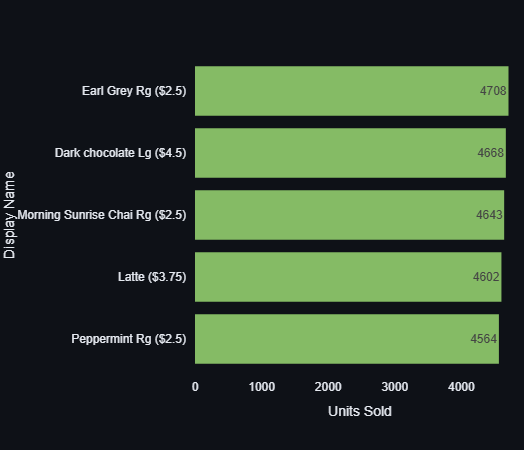
\includegraphics[width=\textwidth]{top5.png}
        \caption{Top 5 Products by Volume}
    \end{minipage}
    \hfill
    \begin{minipage}{0.48\textwidth}
        \centering
        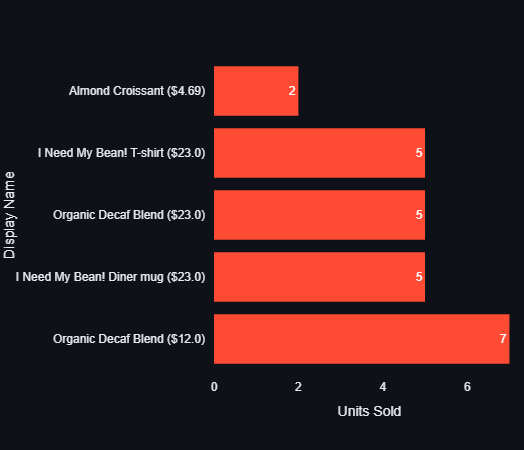
\includegraphics[width=\textwidth]{bottom5.png}
        \caption{Bottom 5 Products by Volume}
    \end{minipage}
\end{figure}

\subsubsection{Revenue Distribution by Product Category}
The fiscal analysis categorizes the total revenue into six primary segments. As shown in Figure \ref{fig:rev_pie}, the business is heavily anchored by beverage sales, with Coffee and Tea combined accounting for 66.7\% of the total intake.

\begin{figure}[H]
    \centering
    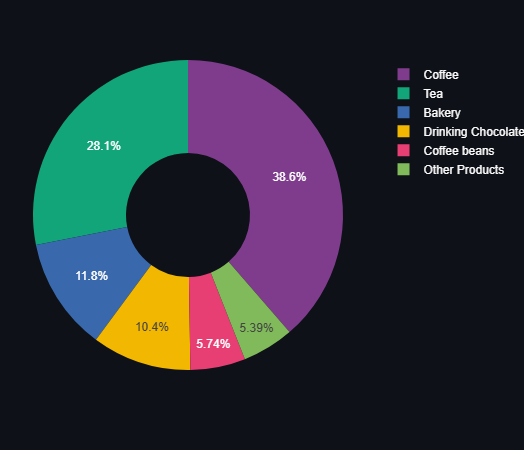
\includegraphics[width=0.7\textwidth]{revpie.png}
    \caption{Revenue Share by Category: Coffee (38.6\%) and Tea (28.1\%) act as the primary pillars of the revenue model.}
    \label{fig:rev_pie}
\end{figure}

\begin{itemize}
    \item \textbf{Coffee (38.6\%):} The dominant category, driven by high-margin Espresso and Brewed variants.
    \item \textbf{Tea (28.1\%):} A significant secondary driver, showing high consumer interest in non-coffee alternatives.
    \item \textbf{Bakery (11.8\%):} Represents the primary cross-selling category, peaking during morning hours.
    \item \textbf{Drinking Chocolate (10.4\%):} A consistent performer within the specialty beverage segment.
    \item \textbf{Ancillary Categories:} Coffee Beans (5.74\%) and Other Products (5.39\%) represent the long-tail retail and merchandise segment.
\end{itemize}


\subsubsection{Menu Engineering and Temporal Trends}
To further optimize the menu, we mapped items onto a popularity-profitability matrix and analyzed hourly demand.

\begin{figure}[H]
    \centering
    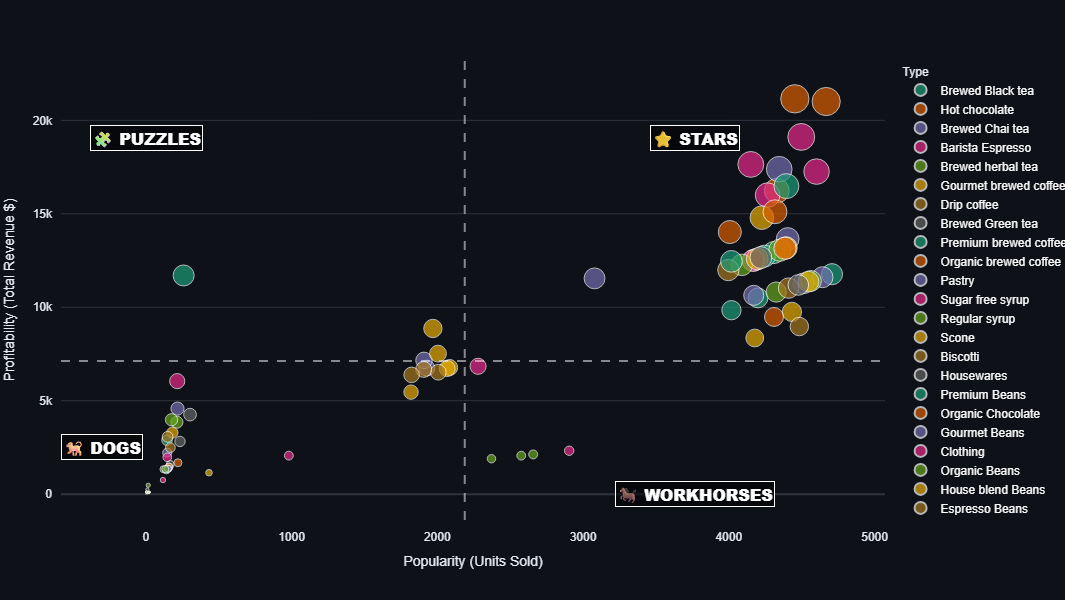
\includegraphics[width=0.85\textwidth]{scatterplot.png}
    \caption{Menu Engineering Matrix: Stars, Puzzles, Workhorses, and Dogs.}
\end{figure}

\begin{figure}[H]
    \centering
    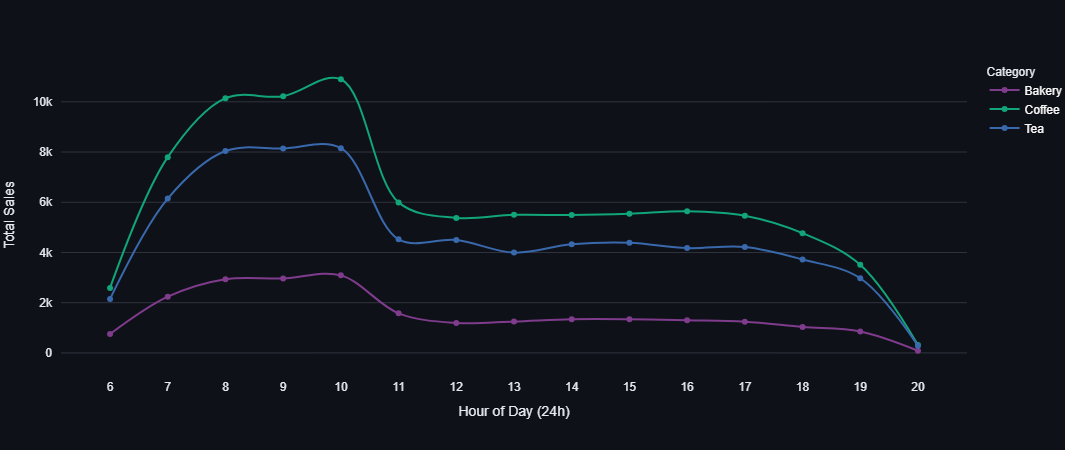
\includegraphics[width=0.9\textwidth]{time.png}
    \caption{Hourly Transaction Volume: Peak demand identified at 10:00 AM.}
\end{figure}
	
	\newpage
\section{Conclusion}
This study successfully developed and deployed a comprehensive Business Intelligence (BI) framework for \textit{Afficionado Coffee Roasters}. By processing 214,470 transactions, we have moved from raw data to actionable strategic insights.

The primary objectives were met through the following findings:
\begin{itemize}
    \item \textbf{Revenue Stability:} The business maintains a healthy revenue concentration ratio of \textbf{42.9\%}, indicating that it is not overly reliant on a single product, though Coffee (38.6\%) and Tea (28.1\%) remain the undisputed pillars.
    \item \textbf{Operational Efficiency:} We identified a critical ``Golden Hour'' between \textbf{08:00 AM and 10:00 AM}, where demand peaks across all categories.
    \item \textbf{Menu Optimization:} The Pareto and Scatter Plot analyses successfully isolated \textbf{56 underperforming products} (Dogs) that contribute to less than 20\% of revenue, providing a clear path for inventory reduction.
\end{itemize}

\section{Strategic Recommendations}
Based on the empirical evidence gathered from the dashboard, the following actions are recommended to the management and stakeholders:

\begin{enumerate}
    \item \textbf{Dynamic Labor Scheduling:} Realign staff shifts to ensure maximum coverage during the 08:00--10:00 AM window. This will reduce wait times and maximize throughput during peak revenue hours.
    \item \textbf{Menu Rationalization:} Phase out the ``Bottom 5'' performers, such as the \textit{Almond Croissant} (2 units sold), and reallocate that shelf space to ``Star'' products like \textit{Earl Grey} and \textit{Barista Espresso}.
    \item \textbf{Bundling Strategy:} Since \textit{Bakery} (11.8\%) is a secondary driver, implement a ``Breakfast Bundle'' (Coffee + Pastry) specifically during the 07:00--09:00 AM slot to increase the Average Transaction Value (currently \$4.69).
    \item \textbf{Inventory Focused Marketing:} Focus marketing efforts on the \textit{Puzzles} quadrant (high profit but lower volume) to shift them into the \textit{Stars} category.
\end{enumerate}

\section{Limitations}
While this study provides a robust data-driven foundation for business strategy, certain constraints must be acknowledged to contextualize the findings:

\begin{itemize}
    \item \textbf{Data Scope:} The analysis is strictly confined to historical transactional records provided by Afficionado Coffee Roasters. As such, it reflects past performance but does not account for real-time inventory fluctuations or supply chain disruptions.
    \item \textbf{Exclusion of External Variables:} High-level external factors—including local competition, shifting market pricing strategies, and broader macroeconomic seasonality—were not integrated into this analytical phase.
    \item \textbf{Observational Nature:} This is an observational study based on existing data; therefore, no causal inference can be definitively drawn. For example, while sales peak at 10:00 AM, the data alone cannot determine if this is due to consumer habits or specific morning-only promotions.
    \item \textbf{Absence of Predictive Modeling:} This phase focused exclusively on Descriptive and Diagnostic Analytics (Exploratory Data Analysis). Predictive modeling for future sales forecasting or churn analysis was not applied in this iteration of the engine.
\end{itemize}

\section*{Digital Deliverables \& BI Access}
To ensure these insights remain dynamic and interactive for stakeholders, the full analytical engine has been published online.
\begin{itemize}
    \item \textbf{Interactive BI Dashboard:} \href{https://afficionado-roasters-bi-dashboard-gxhznyk5jednzcbb5hhygk.streamlit.app/}{Access Live Analytics Here}
    \item \textbf{Source Code Repository:} \href{https://github.com/Debayanmal2002-official/Afficionado-Roasters-BI-Dashboard}{View Project on GitHub}
\end{itemize}
	
\end{document}
